\documentclass[a4paper,12pt,reqno]{article}
\usepackage{amsfonts}
\usepackage{graphicx}
\usepackage{geometry}
\usepackage{color}
\usepackage{amssymb,amsmath}
\usepackage{polski}
\usepackage[T1]{fontenc}
\usepackage[utf8]{inputenc}
\usepackage{caption}
\geometry{margin=1.1in}
\usepackage{wrapfig}
\usepackage{lipsum}  
\usepackage{listings}
\usepackage[toc,page]{appendix}

\definecolor{codegreen}{rgb}{0.5, 0.09, 0.09}
\definecolor{codegray}{rgb}{0.5,0.5,0.5}
\definecolor{codepurple}{rgb}{0.58,0,0.82}
\definecolor{backcolour}{rgb}{0.94,0.94,0.94}
\definecolor{gray}{rgb}{0,0.6,0}

\lstdefinestyle{mystyle}{
    backgroundcolor=\color{backcolour},  
    commentstyle=\color{codegreen},
    keywordstyle=\color{blue},
    numberstyle=\tiny\color{codegray},
    stringstyle=\color{codepurple},
		basicstyle=\footnotesize\fontfamily{cmtt}\selectfont,
    breakatwhitespace=false,         
    breaklines=true,
    captionpos=b,
		language=C++,
    keepspaces=true,                 
    numbers=left,                    
    numbersep=5pt,                  
    showspaces=false,                
    showstringspaces=false,
    showtabs=false,                  
    tabsize=2
}
 
\lstset{style=mystyle}
\lstset{literate=%
    *{0}{{{\color{gray}0}}}1
    {1}{{{\color{gray}1}}}1
    {2}{{{\color{gray}2}}}1
    {3}{{{\color{gray}3}}}1
    {4}{{{\color{gray}4}}}1
    {5}{{{\color{gray}5}}}1
    {6}{{{\color{gray}6}}}1
    {7}{{{\color{gray}7}}}1
    {8}{{{\color{gray}8}}}1
    {9}{{{\color{gray}9}}}1
}
%------------------------------------------------------------
\begin{document}



\begin{center}

\thispagestyle{empty}

\Large 
\vspace{0.8cm}
\vspace{1.8cm}

\Large Krystian Skibiński \\
\vspace{3.2cm}
\Large Emulator maszyny wirtualnej CHIP-8 \\
CHIP-8 virtual machine emulator
\end{center}
\vspace{15.7cm}
\begin{center}
\small Publiczna wersja pracy inżynierskiej nie posiada ona żadnych danych uniwersytetu.
\end{center}

\vspace{1.2cm}

\begin{center}
\large Wrocław, 2019
\end{center}

\newpage

\tableofcontents

\newpage

\begin{flushleft}
\Large \textbf{Streszczenie}
\end{flushleft}
\vspace{1cm}

 Celem pracy jest przygotowanie interpretera maszyny wirtualnej CHIP-8, za pomocą którego możliwe będzie emulowanie programów napisanych dla tego komputera. Projekt zostanie zrealizowany przy użyciu języka skryptowego - Python wraz z wykorzystaniem biblioteki Tkinter oraz dokumentacją i testami.

\newpage
\begin{flushleft}
\Large \textbf{Abstract}
\end{flushleft}
\vspace{1cm}

 PyChip8 is a CHIP-8 computer interpreter written in Python, which allows you to run programs prepared for this machine directly on your computer.

\newpage

\section{Wstęp}
W dobie błyskawicznego rozwoju internetu i komputerów, maszyny potrzebne do przetwarzania dużych porcji informacji są coraz bardziej skomplikowane. Z jednej strony, ważne są jak najmniejsze rozmiary tych urządzeń, z drugiej ceni się ich wydajność. To prowadzi do tworzenia coraz bardziej skomplikowanych podzespołów i systemów je napędzających. Przeciętna instrukcja komputera z lat 80. zajmowała około 150 stron\footnote{Instrukcja dla programistów najpopularniejszego komputera lat 80 - Commodore 64 zawiera 491 strony \cite{Commodore}.}, a jej zawartość opisywała budowę i działanie urządzenia, włącznie z zaprezentowaniem wszystkich instrukcji wbudowanego języka programowania, wyświetlaniem i manipulacją grafiki, czy dźwięku. Dzisiejsze instrukcje dla samych procesorów zawierają 5000 stron\footnote{Instrukcja dla projektantów oprogramowania, procesora Intel o architekturze i32 zawiera 4670 stron \cite{Intel}.}, a jest to jeden z elementów jednostki centralnej, poza tym pozostaje jeszcze system. Z tego powodu współczesne tworzenie oprogramowania opiera się na jeszcze większej abstrakcji, zestawach bibliotek i narzędzi. Nie mniej znajomość działania procesora, czy pamięci komputera, nadal stanowi istotną kwestie, dla twórców oprogramowania i inżynierów. Pod warstwą obecnie dostarczanych, modułów i pakietów, nadal są przeprowadzane typowe dla wczesnych komputerów operacje. Stanowią one dobre źródło do tego, aby zagłębić się w budowę współczesnych architektur. \\

Projekt ten powstał w celach hobbistycznych, jako wynik fascynacji 8-bitowymi komputerami i chęci zbudowania własnej jednostki. Jego założeniem jest przybliżenie użytkownikowi działania prostej architektury wczesnych elektronicznych maszyn cyfrowych. Dlatego został on upubliczniony jako \textit{wolne oprogramowanie} w serwisie \textit{github \footnote{Adres do repozytorium: github.com/krskibin/pyChip8 }} na \textit{licencji MIT\footnote{Więcej o licencji \textit{MIT} na stronie: https://opensource.org/licenses/MIT}}. W jego ramach było przygotowanie emulatora maszyny wirtualnej CHIP-8. Opracowany program działa jako aplikacja okienkowa, która odtwarza napisane w tym języku pliki binarne, wraz z emulacją grafiki, dźwięku i obsługą klawiatury. \\

W rozdziale drugim została poruszona kwestia komputerów 8-bitowych, ich historia, w tym również omawianej maszyny wirtualnej CHIP-8. Następnie w rozdziale trzecim przedstawiono zagadnienia teoretyczne związane z pracą. Na początku omówiono maszynę wirtualną, związane z nią zagadnienia, takie jak emulacja, czy wirtualizacją, przedstawiono różnicę między tymi pojęciami, następnie opisano zagadnienia potrzebne do opracowania własnego emulatora, takie jak przesunięcia bitowe, stosy, czy rejestry. Rozdział czwarty został poświęcony specyfikacji omawianego CHIP-8, jest to abstrakcyjna instrukcja, którą musiał spełniać komputer, na którym chciano zaimplementować ten system. W tym rozdziale poruszono budowę jego pamięci, procesora, wspieranych urządzeń wejścia, wyjścia. W rozdziale piątym przedstawiono specyfikację projektu, to jakie problemy niesie za sobą budowa emulatora, jego architekturę, strukturę klas, a także wymagania funkcyjne i niefunkcyjne, wraz z schematami użycia stworzonego programu. Następnie w rozdziale szóstym zawarto implementacje projektu, opisano proces budowy poszczególnych elementów maszyny wirtualnej, a także przedstawiono implementacje niektórych z instrukcji procesora. Rozdział siódmy poświęcony był napisanym testom. Pokrótce zaprezentowana została ich struktura i omówiona najważniejsze techniki odpowiedzialne za ich poprawne przygotowanie. Rozdział ósmy, to z kolei, podsumowanie pracy, a także przedstawienie kolejnych etapów jej rozwoju.
\section{Komputery 8-bitowe}
\subsection{Architektura 8-bitowa}
To architektura komputera, w której używa się 8-bitowych rejestrów, jednostek \\arytmetyczno-logicznych i komórek pamięci \cite{Stakem}. Ta ilość danych była jednak niewystarczająca przy adresowaniu pamięci, dlatego komputery te posiadały najczęściej 16-bitową \textit{szynę pamięci} \cite{Stakem}, która pozwala na indeksowanie komórek do \textit{64kB~\footnote{Pamięć była maksymalnie adresowana od 0 do $2^{16}$ czyli 65536 bitów.}}. Wówczas rozszerzano, również wielkość instrukcji i niektórych rejestrów do wartości 16-bitowych.

\subsection{Historia}
Rozwój komputerów rozpoczął się na dobre po drugiej wojnie światowej. W 1947 roku został wynaleziony tranzystor bipolarny, który od 1955 roku zaczął zastępować duże lampy elektronowe, znacząco zmniejszając rozmiary komputerów. Odtąd tranzystory mogły posiadać tysiące bramek logicznych przy relatywnie małym zużyciu miejsca. Następnym wielkim odkryciem, było wprowadzenie układów scalonych. Jack Kilby opracował pierwszy działający czip. Pół roku później Robert Noyce \cite{Petzold}, zaprezentował swój układ, w którym rozwiązał wiele problemów jego konkurenta, największą zmianą było zastosowanie krzemu, zamiast germanu. Rozpoczęły się wyścigi firm technologicznych, aby stworzyć jak mniej zasobożerne jednostki. W 1968 roku Noyce wraz z Gordon E. Moore'em (późniejszym twórcą prawa Moore'a) otwierają firmę \textit{Intel}, zaledwie trzy lata później wypuszczają na rynek pierwszy komercyjny \cite{Stakem} mikroprocesor \textit{Intel 4004}, który z uwagi na małą moc obliczeniową trafia głównie do kalkulatorów \cite{Petzold}, jednak jego twórcy pozostawiają innym możliwość jego przeprogramowania. Dało możliwość pierwszym hobbistom elektroniki na wykorzystanie tych czipów we własnym zakresie. Dopiero drugi produkt \textit{Intela} przyniósł rewolucję. Zrezygnowano z architektury 4-bitowej na rzecz 8-bitowej, która w tamtych czasach była jedynie opracowana teoretycznie. \textit{Intel 8008} ugruntował pozycje firmy i przyniósł ogromne zyski. Pierwotnie procesor był zaprojektowany dla firmy \textit{CTC}, która chciała ich użyć do swoich terminali. \textit{Datapoint 2200} \cite{Stakem} miał służyć do odczytywania danych z jednostek typu mainframe, czyli ogromnych stacji służących do krytycznych obliczeń finansowych lub statystycznych. Dzięki wykorzystaniu charakterystyki dostarczonej przez swoich  partnerów, firma z Santa Clara opracowała technologię, która mogła napędzić pierwsze komputery osobiste. \\

 Zanim jeszcze zaczęto sprzedawać pierwsze produkty \textit{Intela}, Joseph Weisbecker w 1971 roku pracował przy projekcie procesora 8-bitowego \cite{Edwards}, który został przerwany po premierze \textit{i4004}. Jednostka sprzedawała się na tyle dobrze, że firma w której pracował Weisbecker, RCA zgodziła na kontynuowanie prac nad własnym czipem. Niedługo potem, zaprezentowano pierwszy procesor tej firmy, stworzony w technologii \textit{CMOS} (ang. \textit{Complementary Metal-Oxide Semiconductor}), złożony z dwóch układów \textit{COSMAC 1801U} i \textit{1801R} \cite{Edwards}, rok później połączono je w jeden chip o nazwie \textit{COSMAC 1802} . W między czasie (1975 rok), Weisbecker wydał zestaw edukacyjny pod nazwą RCA Microtut, zestaw do samodzielnego złożenia (ang. \textit{Do-It-Yourself Computer}), który miał uczyć podstaw budowy komputera i programowania. Niedługo później \textit{RCA} wydało konsole \textit{RCA Studio II}, powstałą na wniosek Weisbeckera. Opierał się na wcześniej wspominanym czipie \textit{COSMAC 1802}. Komputer nie odniósł większego sukcesu, prawdopodobnie z uwagi na brak kontrolerów, zamiast, których użyto klawiatury heksadecymalnej \cite{Cowgod}. Sprzęt ten posłużył córce Josepha, Joyce Weisbecker, która nauczyła się programować dzięki tej konsoli. W historii zapisała się jako pierwsza kobieta, która tworzyła gry komercyjne \cite{Edwards}. W 1976 roku czasopismo \textit{Popular Electronics} wydało opracowanych przez Weisbeckera schemat budowy komputera \textit{COSMAC ELF}, będącą blisko powiązaną z \textit{Microtut}jednostką zaprojektowaną dla hobbistów, którzy bez większych przeszkód mogli złożyć go w swoim domu. W późniejszej serii magazyn dodał do urządzenia prostą kartę graficzną opartą o tę z konsol \textit{Studio II} \cite{Edwards}. W tym samym roku \textit{RCA}, oddało do sprzedaży następny komputer, \textit{COSMAC VIP}, który w głównej mierze opierał się na \textit{COSMAC ELF}. Posiadał on wbudowany język programowania zaprojektowany przez Weisbeckera - CHIP-8 \cite{Cowgod}.
 


\section{Emulacja}
\subsection{Wirtualizacja, a emulacja}
Pomimo swojej złożoności systemy komputerowe nadal ewoluują, jest to możliwe dzięki dobrze zaprojektowanym interfejsom, które oddzielają poziomy abstrakcji, przez co niepotrzebna jest szczegółowa znajomość implementacji niższego poziomu, ułatwia to w niezależny sposób rozwój warstwy sprzętowej jak i oprogramowania. Niestety ma to swoje ograniczenia, aplikacje, które są dystrybuowane jako skomplikowane pliki binarne zależą od konkretnego interfejsu systemu operacyjnego \cite{James}. Istnieją dwie główne metody, które zapewniają sposób na obejście takich ograniczeń. Pierwsza z nich to wirtualizacja. Jej zadaniem jest ominięcie warstwy sprzętowej lub systemowej i odpowiednie jej zmapowanie na inny system lub architekturę sprzętową. Sam koncept wirtualizacji nie musi wyłącznie odnosić się do poszczególnych podzespołów lub podsystemów, ale do całych maszyn. Wówczas programiści muszą dostarczyć oprogramowanie, które wspiera całą architekturę urządzenia\cite{James, Popek}, tworząc w ten sposób maszynę wirtualną. Dzięki temu omijają oni rzeczywistą kompatybilność urządzeń, jaki i ograniczenia zasobów sprzętowych. Innym podejściem na wyabstrahowanie jednego systemu w drugim jest emulacja, która w swoich założeniach również opiera się na maszynie wirtualnej, ale zamiast dostarczać wirtualne interfejsy jak w przypadku wirtualizacji, symuluje działanie całej architektury urządzenia. Główna różnica polega na tym, że w pierwszym przypadku zestaw instrukcji procesora (\textit{ISA}) gospodarza \cite{James} jest taki sam, lub w większości podobny do tego w maszynie wirtualnej. Niepasujące do zestawu hosta kody procesora są przechwytywane i wykonywane przez oprogramowanie \cite{ROSENTHAL}. Z kolei podczas emulacji implementuje się maszynę wirtualną na komputerze gospodarza, którego zestaw instrukcji jest inny od tego z bazowego sprzętu (gościa). W tym przypadku żadna z instrukcji nie jest bezpośrednio przetwarzana przez procesor gospodarza, tylko interpretowana, za pomocą specjalnego programu (interpretera) \cite{James}. Wyodrębnia on każdy ciąg bitów, następnie odkodowuje i emuluje ich wykonanie. Oprogramowanie hosta, które wykonuje tę interpretacje, naśladując zestaw instrukcji maszyny wirtualnej i jej wirtualną konfigurację sprzętową, jest nazywane emulatorem \cite{ROSENTHAL}. Niestety cały ten proces jest relatywnie wolny. W latach 70, twierdzono nawet, że emulacja nie jest powiązana z tworzeniem maszyny wirtualnej, ponieważ proces ten nie jest wystarczająco wydajny, aby mógł on dostatecznie symulować działanie danego urządzenia \cite{Popek}:
\begin{quotation}
"The second characteristic of a virtual machine monitor is efficiency. It demands that a statistically dominant subset of the virtual processor's instructions be executed directly by the real processor, with no software intervention by the VMM. This statement rules out traditional emulators and complete software interpreters (simulators) from the virtual machine umbrella."
\end{quotation}
Jednak z początkiem lat 90. coraz popularniejsze stawały się komputery oparte na architekturze 32-bitowej, które z łatwością mogły emulować 8-bitowe systemy z końca lat 70.

\subsection{Bity i bajty}
Pomimo swojej złożoności, istotą komputera jest przetwarzanie informacji. To elektryczna maszyna, która może rozpoznać tylko dwa stany napięciowe; brak lub bardzo niskie napięcie i wysokie napięcie, generując przy tym sygnał ciągły (analogowy), który zamieniany jest na sygnał cyfrowy, czyli skwantowany. Przyjęto, że sygnał ten będzie reprezentowany w formie zero-jedynkowej, jeden gdy napięcie jest wysokie i zero gdy jest niskie. Taki system przedstawiania cyfr nazywany jest dwójkowym lub binarnym. Już jedna liczba binarna może przedstawić, w którym z dwóch możliwych stanów jest dany układ, dlatego jest ona uznawana za najmniejszą cząstkę informacji możliwą do przetworzenia przez komputer, dzięki czemu zyskała miano bitu. Inną z podstawowych funkcji komputera jest możliwość przechowywania informacji. Dawniej zdecydowano, że najmniejszą ilością przechowywanych bitów  w jednym adresie komórki pamięci będzie bajt, który z początku nie miał określonej liczby \cite{Petzold}, dopiero później ustalono, że będzie to 8 bitów. Natomiast, bity o określonej długości na których operacje wykonuje procesor nazwano \textit{słowem}. Jeśli słowo tworzą 32 bity, to taki procesor określany jest jako 32-bitowy. Niestety, przy dużej ilości danych generowanych przez komputery ich przedstawianie za pomocą systemu dwójkowego nie jest czytelne dla człowieka. Ze względu na chęć zachowania większej zwięzłości, w literaturze informatycznej, zdecydowano na zapisywanie ich za pomocą systemu szesnastkowego \cite{Petzold}. \\

Użycie systemu szesnastkowego ułatwia identyfikowanie poszczególnych komórek pamięci czy wartości rejestrów. \\Wszystkie instrukcje przetwarzane przez procesor CHIP-8, również są zapisane w takiej formie. Dzięki temu osoby piszące oprogramowanie na tę jednostkę zamiast używać \textit{słów} o długości 16 bitów, mogą z powodzeniem zapisywać je w formie czteroznakowej. Dodatkowo w instrukcji \cite{COSMAC} zastosowano podział na mniejsze jednostki informacji niż bajty. \\

Do reprezentacji 4-bitowej (jeden znak w systemie szesnastkowym) użyto \textit{półbajta} (ang. \textit{nibble}, \textit{nybble}), z czego bity 7-4 nazywane są \textit{młodszymi}, a bity 0-3 \textit{starszymi} \cite{Cowgod}. Aby łatwiej było identyfikować różne rejestry w jednej instrukcji, wprowadzono oznaczenia \textit{x}, dla młodszych bitów pierwszego bajtu kodu procesora i \textit{y} dla starszych bitów drugiego. Z kolei wartość 12-bitowa jest określana jako adres, ponieważ za jej pomocą identyfikuje się komórki pamięci w komputerze. \\

\subsection{Operatory binarne}
Operowanie na informacji przez procesor nie sprowadza się jedynie do prostych działań matematycznych. Jednostka obliczeniowa wykonuje też operacje binarne, które nie tylko służą programistom do manipulacji zmiennymi, ale również wykorzystywane są przez sam procesor do odpowiedniego pozyskiwania i interpretowania instrukcji. Wśród operatorów bitowych dostępnych w większości współczesnych języków programowania można wyróżnić, \textit{jednoargumentowe}, do których należy negacja, reprezentowana najczęściej za pomocą tyldy ("$\sim$"), lub te wieloargumentowe w skład których wchodzą: koniunkcja ("\&"), alternatywa ("|"), alternatywa wykluczająca ("\string^"), przesunięcia bitowe ('>>' lub '<<'). \\

\subsection{Asembler i deasembler}
W związku z tym, że każdy zestaw kodów operacyjnych dla procesorów różni się w zależności od ich architektury i producenta, powstała cała grupa niskopoziomowych języków programowania nazywana \textit{językami asemblera}, w których każda instrukcja jest mnemonikiem\footnote{Posiada ona uproszczoną słowną reprezentacje czynności procesora} kodu procesora. Proces zamiany zrozumiałego dla człowieka kodu na maszynowy jest dokonywany za pomocą specjalnego programu, który nazywany jest \textit{asemblerem}. Instrukcja \textit{COSMAC VIP} \cite{SCHWARZ} nie posiada składni dla języka assemblera, jednak w \textit{Cowgod's Chip-8 Technical Reference} zamieszczone zostały mnemoniczne nazwy poszczególnych instrukcji, które posłużą do nazwania odpowiadających im funkcji w projekcie emulatora. Dobrą praktyką jest tworzenie programów nazywanych deasemblerami, które przetwarzają kod pliku binarnego na ten w postaci mnemonicznej, zrozumiałej dla człowieka. Ich podstawowym celem jest dokładniejsze zrozumienie działania emulowanego urządzenia. Tego typu programy często stanowią podstawę dla pełnoprawnego emulatora. \\

\subsection{Rejestry i stosy}
Rejestry są to pojemniki na dane o niewielkich rozmiarach służące do przetrzymywania krótkotrwałego wyniku operacji, adresów lokacji w pamięci operacyjnej itd. Dostęp do nich, w porównaniu między innymi do pamięci RAM, jest błyskawiczny \cite{Coldwin}. Procesory najczęściej posiadają kilka rodzajów rejestrów, różniące się one zastosowaniem. W projekcie zostały użyte, te ogólnego przeznaczenia, służące głównie do przetrzymywania wyników operacji arytmetyczno-logicznych na liczbach naturalnych i rejestry specjalne w skład których wchodzą rejestry sterujące (sterujące zachowaniem procesora) i rejestry stanu (przechowujące informacje np. o wystąpieniu pewnego rodzaju zdarzenia)~\cite{Coldwin}. \\

Innym z ważnych elementów budowy procesora jest stos, którego zadaniem jest  zapis tymczasowych danych, takich jak argumenty funkcji, zmienne lokalne, adresy powrotów z funkcji itp. Zasada jego działania opiera się na znanej z algorytmiki strukturze danych o tej samej nazwie. Jednostka obliczeniowa za pomocą rejestru nazywanego wskaźnikiem stosu (ang. \textit{stack pointer}) \cite{Coldwin} steruje jego rozmiarem i przy  wykonaniu odpowiedniej instrukcji dodaje lub usuwa wskazywaną wartość inkrementując lub dekrementując przy tym jego wskaźnik. Zasada ta jest określona jako \textit{LIFO}(ang. \textit{First In Last Out})~\cite{Cormen}. Ostatni dodany element do stosu jest, tym, który jako pierwszy zostanie z niego usunięty.

\subsection{Procesor}
Procesor jest jednostką w maszynie odpowiedzialną za wykonywanie podstawowych operacji. Natomiast rejestry można przyrównać do zmiennych w językach programowania. CHIP-8 posiada ich kilka (V0 - VF), można je potraktować
jak zmienne w języku C++:
\begin{lstlisting}[language=c]
unsigned char V0, V1, V2, V3, V4 ... VF;
\end{lstlisting}
Procesory posiadają także program counter (PC), który można potraktować jako znany z języków, wskaźnik:
\begin{lstlisting}[language=c]
unsigned char *pc;
\end{lstlisting}
To jaki ciąg liczb odpowiada danej instrukcji zapisane jest między innymi w dokumentacji technicznej do CHIP-8 \cite{Cowgod}. Dla przykładu, gdy program counter wskazuje na 0x8FC0, to wykonywana jest instrukcja LOAD(VF, VC). Wartość rejestru VF przeniesiona zostaje do rejestru VC, odpowiada to asemblerowej operacji MOV, lub w \textit{języku C}: VF = VC. Gdyby \textit{pointer couter} wskazywał na wartość 0x8FC4, to została by wykonana instrukcja ADD, która w \textit{języku asemblera} , jej odpowiednik w \textit{C} to VF = VF + VC. \\

Kolejną ważną kwestią jest czas wykonywania instrukcji. Realizacja każdego kodu procesora w CHIP-8 mierzona jest za pomocą tak zwanych cykli. We współczesnych jednostkach obliczeniowych zależy ona od ilości wykonywanych instrukcji, natomiast w starszych takich jak \textit{COSMAC-1802} czas ten był z góry określony przez producenta urządzenia \textit{Cowgod}. \\
\section{Specyfikacja CHIP-8}
 CHIP-8 jest to interpretowany język programowania oryginalnie zaprojektowany dla komputerów DIY późnych lat 70 i wczesnych 80. Jego główną ideą było uczynienie procesu tworzenia gier łatwiejszym, a także danie możliwości przenoszenia kodu na różne maszyny. W tym celu opracowane zostało specjalne środowisko uruchomieniowe nazywane maszyną wirtualną. Jego schemat jest ogólnodostępny i dobrze udokumentowany. Język ten nie odniósł większego sukcesu jako stricte komputerowy. Stał on się przede wszystkim głównym oprogramowaniem dla mniejszych urządzeń w latach 80. i 90. szczególnie dla kalkulatorów. Najbardziej znanym modelem jest \textit{TI-83}, wydany przez \textit{Texas Instruments}, do zaawansowanych obliczeń naukowych \cite{Cowgod}.

\subsection{Pamięć}
 Język CHIP-8 jest kompatybilny z pamięcią \textit{RAM} do 4KB (4086B), której lokalizacja zaczyna się od adresu 0x000 (0) i kończy na 0xFFF (4096). Pierwsze 512 (0x000 - 0x1FF) bajtów odnoszą się do interpretera i nie są używane przez żadne inne programy, które w większości wczytywane są do pamięci od następnego bajtu (0x200), choć zdarzają się również takie, które wczytywane są dopiero przy 1536 (0x600) bajcie.

\subsection{Rejestry}
  CHIP-8 posiada 8-bitowe rejestry ogólnego przeznaczenia. Ich nazwy zaczynają się od \textit{V}, a następnie jest im przypisana kolejna cyfra heksadecymalna, co daje szesnaście rejestrów (V0-VF), z tym, że rejestr VF jest używany jako flaga dla niektórych instrukcji, dlatego nie powinien być wykorzystywany. Przygotowano także 16-bitowy rejestr nazywany \textit{I} służący głównie do przechowywania adresów pamięci. Warto wspomnieć o dwóch 8-bitowych rejestrach specjalnego przeznaczenia są one wykorzystywane do trzymania stanu dla opóźniacza (ang. delay) i czasomierza. Są one automatycznie obniżane co 60Hz. Istnieją jeszcze tak zwane \textit{pseduo-rejestry} do których nie ma dostępu z wykonywanych programów. Jeden z nich \textit{program counter} (16-bitowy), trzyma adres obecnie wykonywanej komórki w pamięci. Kolejny, \textit{stack pointer} (8-bitowy) jest używany do wskazywania najwyższego poziomu kopca. Natomiast kopiec to tablica szesnastu elementów po 16-bitów, w której trzymane są adresy. Powinny one zostać zwrócone po zakończeniu danego podprogramu (eng. \textit{subroutine}). CHIP-8 pozwala na działanie do szesnastu zagnieżdżonych podprogramów. 

\subsection{Klawiatura}
Układ klawiszy obsługiwanych przez maszynę wirtualną CHIP-8, odpowiada temu wykorzystanemu w komputerze \textit{COSMAC VIP}. Posiada on klawiaturę heksadecymalną, której schemat znajduje się poniżej:
\begin{table}[h!]
 \centering
 \caption{Układ klawiszy CHIP-8}
 \label{C8Keyboard}
 \begin{tabular}{|c|c|c|c|}
   \hline 
   1 & 2 & 3 & C\\
   \hline
   4 & 5 & 6 & D\\
   \hline
   7 & 8 & 9 & E\\
   \hline
   A & 0 & B & F\\
   \hline
 \end{tabular} 
\end{table}
\newpage
\subsection{Ekran}
 W oryginalnej implementacji języka CHIP-8 został użyty monochromatyczny ekran o rozmiarze 64x32-piksele. Każdy piksel identyfikowany jest za pomocą współrzędnych \textit{x}, \textit{y}, których numeracja zaczyna się w lewym górnym rogu ekranu. 

\begin{table}[h!]
  \centering
  \caption{Format ekranu}
  \label{C8Display}
  \begin{tabular}{|c c|}
    \hline 
    (0, 0) & (63, 0)\\ [1ex] 
    (0, 31) & (63, 31)\\ 
    \hline
  \end{tabular} 
\end{table}

Obraz rysowany jest poprzez tak zwane duszki (ang. \textit{sprite}), czyli grupie bajtów odpowiadających binarnej reprezentacji obrazu. Mogą one mieć wielkość do 15 bajtów, co przekłada się na maksymalny rozmiar 8x15 pikseli.\\

Dodatkowo programy wczytane do pamięci urządzenia mogą odnosić się do duszków reprezentujących notacje szesnastkową, czyli znaków od \textit{0} do \textit{F}. Ich dane w postaci heksadecymalnej powinny znajdować się w obszarze pamięci interpretera (adresy od 0x000 do 0x1FF), po włączeniu urządzenia.


\subsection{Dźwięk i zegary}
 W swojej pierwotnej implementacji komputer posiada dwa zegary, jeden służy do opóźnień (ang. \textit{delay timer}), a drugi do sterowania dźwiękiem. Oba zegary aktywne są tylko wtedy, gdy ich rejestry mają wartość większą od zera. Zadaniem pierwszego z nich jest jedynie odejmowanie jedynki z wartości trzymanej w rejestrze DT przy częstotliwości 60Hz. Drugi natomiast robi dokładnie to samo, również odejmując jeden od wartości w rejestrze ST przy dokładnie tej samej częstotliwości. Różnica polega na tym, że w chwili dekrementacji wartości trzymanej w rejestrze, zegar ten uruchamia zamontowany w komputerze brzęczyk. Ma on tylko jeden ton, a jego zakres nie jest nigdzie podany i zależy wyłącznie od autora interpretera.
 
\subsection{Instrukcje procesora}
Język CHIP-8 posiada 36 różnych instrukcji odnoszących się do działań matematycznych, obsługi grafiki i sterowania wykonywaniem programu. Każda z nich składa się z dwóch bajtów, z czego ten najbardziej znaczący musi być przechowywany w parzyście zaadresowanej komórce pamięci \textit{RAM}. Bajty ładowanych duszów muszą być dopełnione tak, aby nie złamać tej zasady. Lista wszystkich dostępnych kodów procesora wraz z ich opisami jest dostępna w instrukcji komputera \textit{COSMAC VIP} \cite{COSMAC} lub w \textit{Cowgod’s Chip-8 Technical Reference} \cite{Cowgod}.
\section{Założenia projektowe}
W tym rozdziale opisane zostały problemy na jakie można natknąć się w trakcie jego implementacji, wraz z wyszczególnieniem dostępnych rozwiązań. Następnie scharakteryzowana została wybrana architektura aplikacji i szczegółowo opisano jej schemat wraz z pakietami wykorzystanymi do jego implementacji. Omówiono również środowisko programistyczne w jakim będzie działać emulator.

\subsection{Opis problemu i dostępnych rozwiązań}
Podstawowym problemem przy projektowaniu emulatora jest implementacja modułu procesora. To on odpowiada za obliczenia, przetwarzanie pamięci \textit{RAM} oraz zarządzanie rejestrami. Jego działanie jest ściśle określone poprzez zestaw instrukcji, które nieodpowiednio przetłumaczone na język programowania, zaburzają działanie całego programu, generując przy tym trudne do odnalezienia błędy. W tym przypadku, sprawdza się dobrze zaprojektowana struktura kodu, oparta na zasadach \textit{KISS} (\textit{ang. \textit{Keep It Simple}}) i \textit{DRY} (\textit{Don't Repeat Yourself}), dbających o zachowanie klarowności kodu projektu. Pomagają w tym równie, testy jednostkowe, które poza tym mogą sprawdzać, czy dany fragment programu zachowuje się tak, jak zaplanował to programista. Nie chronią one jednak przed błędami wynikającymi ze nieścisłości w  napisanej specyfikacji technicznej, czy też jej niewłaściwym zrozumieniem. Dlatego, aby dobrze zapoznać się z instrukcjami CHIP-8 warto dopisać moduł zajmujący się deasembleracją kodu bitowego wczytanego z programu działającego na tę platformę, będzie on również pomocny przy ewentualnym odnajdywania błędów emulatora. Inną dobrą praktyką jest implementacja własnego debuggera, który na bierząco wskazywałby na wykonywaną instrukcję, a także wyświetlałby bieżący stan rejestrów.
Emulator musi posiadać moduł odpowiedzialny za wyświetlanie grafiki, dźwięki i obsługę urządzeń wejścia. Istnieje wiele dostępnych pakietów napisanych w języku Python, takich jak Tkinter, PyQT oraz wxWidgets nadających się do implementacji tych funkcji. Dobrym rozwiązaniem jest także wykorzystanie bibliotek odpowiedzialnych za grafikę, takich jak pyglet, bezpośrednio odnoszących się do OpenGL lub skierowanych do tworzenia gier: pygame, arcade.
Istotnym problemem jest również interakcja z użytkownikiem i dostarczenie mu interfejsu do wczytywania \textit{obrazów ROM}.

\subsection{Architektura systemu}
Architektura aplikacji została przemyślana tak, aby każdy z modułów odpowiadał za inną funkcje, oddzielając poszczególne warstwy abstrakcji. Komponent odpowiedzialny za pamięć, przechowuje wczytane dane, które następnie są przetwarzane przez moduł symulujący jednostkę obliczeniową i wyświetlane użytkownikowi w warstwie \textit{wyjścia/wejścia}. Zewnętrzne interakcje są również przekazywane przez warstwę prezentacji do opracowania przez procesor, a przy chęci zmiany wczytanego przez emulator programu, żądanie to trafia do procesora, który następnie usuwa dane trzymane w module pamięci. Koncepcji tej odpowiada \textit{architektura warstwowa} \cite{Richards}.

\begin{figure*}[!htb]
\begin{center}
	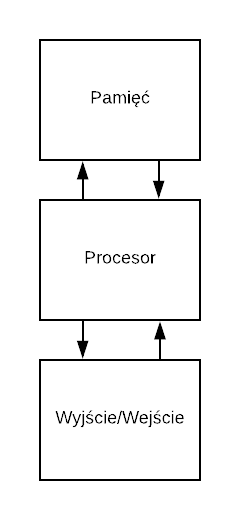
\includegraphics[scale=0.4]{images/architectureDiag}
	\caption{Uproszczony diagram architektury systemu}
\end{center}
\end{figure*}

\newpage

\subsection{Struktura klas}
Struktura klas została oparta na \textit{agregacji}, czyli relacji, która charakteryzuje się, tym, że jeden obiekt jest właścicielem kolejnego, może być on również współdzielony. Klasy \textit{Processor} i \textit{Disassembler} posiadają atrybut o nazwie \textit{memory}, który przechowuje instancje klasy \textit{Memory}. Podobnie jest z strukturą obiektu \textit{Screen}, gdzie pole \textit{proc}, trzyma instancje \textit{Processor}, która dodatkowo jest współdzielona z klasą \textit{Window}. Z kolei relacja między tymi klasami to \textit{kompozycja}. Charakteryzuje się ona tym, że obiekt zagregowany ma taki sam czas życia jak jego właściciel, dodatkowo jego istnienie poza nim nie ma sensu \cite{Trybulec}. \\

Dla uproszczenia na diagramie poniżej nie ma wypisanych metod związanych z obsługą instrukcji procesora, ze względu na ich ilość. Są one oznaczone jedynie jako \textit{instruction functions}. Na schemacie nie ma również graficznego odniesienia do biblioteki \textit{tkinter}. Relacja. dziedziczenia pomiędzy nią, a obiektem \textit{Window} została zasygnalizowana w nawiasach obok nazwy klasy.

\begin{figure*}[!htb]
\begin{center}
	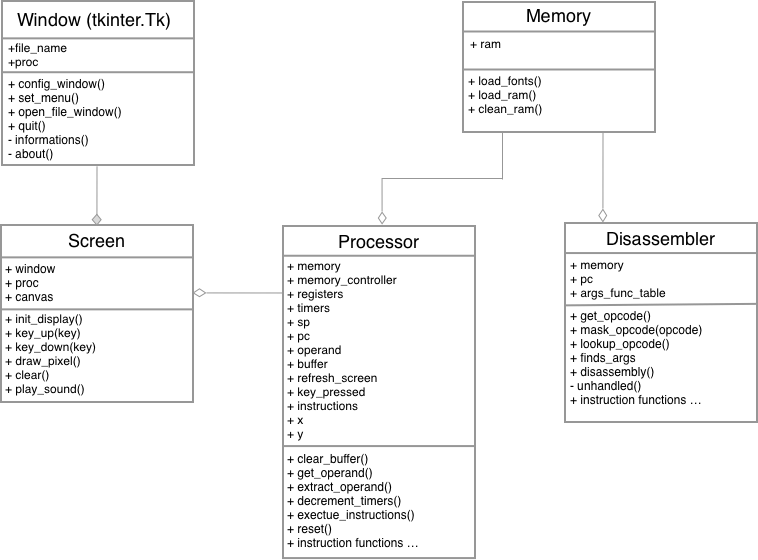
\includegraphics[scale=0.4]{images/class_scheme}
	\caption{Uproszczony diagram schematu klas}
\end{center}
\end{figure*}

\subsection{Wykorzystane biblioteki}
W celu napisania projektu wykorzystano następuje biblioteki:
\begin{itemize}
	\item \textit{Tkinter}, jest to zorientowany obiektowo pakiet napisany jako warstwa dla języka Tcl/Tk \cite{TKINTER}. Dostarcza on niezależne od systemu operacyjnego narzędzia do tworzenia aplikacji okienkowych, włącznie z obsługą multimediów i urządzeń wejścia, takich jak klawiatura, czy mysz komputerowa. Moduł ten od wersji języka Python 3.0 zawiera się \textit{Standardowej Bibliotece Pythona} \footnote{Zestaw pakietów i modułów dostarczanych wraz z instalatorem języka Python, ich wykaz dostępny jest pod adresem: https://docs.python.org/3/library/} i nie wymaga dodatkowej instalacji.
	\item \textit{Pytest} - to zewnętrzne (nie należy do Standardowej Biblioteki języka Python) narzędzie do testowania aplikacji. Jego dokładny opis i zastosowanie zostało zaprezentowane w rozdziale poświęconym testowaniu projektu.
	\item \textit{Pipenv/virtualenv} - zarówno \textit{pipenv}, jaki i \textit{virtualenv} to pakiety służące do tworzenia odizolowanych środowisk programistycznych, dzięki którym możliwe jest instalowanie dowolnych pakietów języka Python bez integracji w pliki systemowe komputera. Pozwala to na korzystanie z różnych wersji paczek zależnie od wymogów projektu w jednym środowisku operacyjnym. \textit{Pipenv} ponadto dostarcza narzędzi, które automatycznie pobierają wymagane paczki, tworzy dla nich wirtualne środowisko i dba o spójność wersji, zapisując plik w którym trzymane są wszystkie zależności, nawet te pośrednie \cite{Reitz}.
	\item \textit{Argparse} - moduł odpowiedzialny za interfejs linii poleceń. Zapewnia obsługę argumentów i opcji podanych przy wywołaniu programu. Dodatkowo automatycznie generuje sekcje \textit{help} i wiadomości o błędach \cite{Argparse}.
\end{itemize}

\subsection{Analiza wymagań}
Projekt informatyczny powinien mieć jasno zdefiniowane wymagania ustalające jego podstawowe funkcje. W rezultacie ma to zapobiec implementacji niepotrzebnych fragmentów kodu i wyszczególnić zestaw cech, które powinien posiadać produkt, aby uznać go za gotowy. Taka analiza zapewnia skupienie się na jasno określonych celach.

\subsubsection{Wymagania funkcyjne}
Zadaniem emulatora jest wczytywanie dostarczonych przez użytkownika plików, \textit{tylko do odczytu}\footnote{z ang. read-only memory, ROM, pamięć, której można jedynie odczytywać, w przypadku emulatorów są pliki binarne (mogą mieć również rozwinięcie .c8, .c8h, ch8 ) lub obrazy gier. }, które będą wczytane do pamięci maszyny wirtualnej. Następnie dane te będą przetwarzane na zaimplementowane instrukcje procesora. W rezultacie, użytkownikowi wyświetli się okno programu, które będzie generować emulowaną grę wraz z możliwością interakcji z nią, dzięki klawiaturze. Ponadto aplikacje będzie odtwarzał dźwięk, a także da użytkownikowi możliwość bezbłędnego przerwania programu lub zresetowania aktualnego stanu maszyny wirtualnej wraz z możliwością zmiany odtwarzanego pliku binarnego. Z dodatkowych funkcji, możliwa będzie także zmiana rozdzielczości, a co za tym idzie rozmiaru okienka wyświetlanego okna i zmiana czasu cyklu procesora, tak aby przyśpieszyć odtwarzany program. Opcje te będą dostępne w menu umieszczonym pod górnym paskiem okienka, a poszczególne z nich będzie również będzie można zmienić uruchamiając program z linii poleceń, dodając do komendy odpowiednie argumenty.

\subsubsection{Wymagania niefunkcyjne}
Emulator będzie ograniczał się do uruchamiania plików jedynie przeznaczonych dla maszyny wirtualnej CHIP-8. Jego wydajność będzie stosunkowo niewielka, ze względu na wybrany język programowania, a także ograniczenia biblioteki \textit{tkinter}. Dodatkowo sama emulacja wiąże się z wykorzystywaniem dużych zasobów pamięciowych (wczytywane pliki są w całości przetrzymywane w pamięci komputera), a także wydajnościowych, gdyż pętla takiego programu, to wykonanie szeregu instrukcji i interakcji, jednak czas ten będzie nadal o wiele szybszy niż podane w specyfikacji taktowanie procesora \cite{Cowgod}.

\subsubsection{Scenariusze użycia}
Scenariusze użycia (ang. \textit{use cases}), to przedstawienie z opisami poszczególnych etapów działania aplikacji w krokach. Mają one na celu uproszczenie wymagań funkcyjnych poprzez ich uporządkowanie. Są również dobrym sposobem do zobrazowania zagrożeń jakie czeka dany system i zaplanowaniem ich kontrolowania. W tym przypadku, zostaną przedstawione wyłącznie scenariusze, gdzie będą istniały ich alternatywne ścieżki. Takie jak zmiana prędkości emulatora, czy rozdzielczości nie mają w założeniu generować alternatywach scenariuszy, dlatego w tym podrozdziale zostaną pominięte.\\

\textbf{UC-01:} Uruchomienie emulatora z linii komend bez podania argumentów\\
\textbf{Aktorzy:} Użytkownik \\
\textbf{Cel:} Uruchomienie aplikacji okienkowej z działającą emulacją wybranego programu, który reaguje na wejście z klawiatury. Dostęp do menu górnego. Po prawidłowym wyłączeniu aplikacja nie zgłasza błędu. \\
\textbf{Główny scenariusz:}
\begin{enumerate}
  \item Aplikacja prezentuje ciemne tło. Z okienkiem informującym o braku wczytanego pliku binarnego.
  \item Użytkownik akceptuje informacje, klikając \textit{OK}, okienko zostaje zamknięte.
  \item Z paska górnego zostaje wybrany \textit{File} > \textit{Open}.
  \item Użytkownik wybiera odpowiedni plik binarny (*, .c8, .ch8).
  \item Program wczytuje plik i wyświetla grafikę.
  \item Użytkownik zakańcza działanie programu poprzez kliknięcie krzyżyka lub opcje w menu.
\end{enumerate}
\textbf{Alternatywny scenariusz:}
\begin{enumerate}
  \item [3a] Użytkownik wybiera niepoprawny plik.
  \item Aplikacja wyświetla błąd \textit"Cannot read file.".
  \item Użytkownik wraca do punktu 2.
\end{enumerate}

\textbf{UC-02:} Uruchomienie emulatora z podaniem nazwy pliku jako argument \\
\textbf{Aktorzy:} Użytkownik \\
\textbf{Cel:} Uruchomienie aplikacji okienkowej z działającą emulacją wybranego programu, który reaguje na wejście z klawiatury. Dostęp do menu górnego. Po prawidłowym wyłączeniu aplikacja nie zgłasza błędu. \\
\textbf{Główny scenariusz:}
\begin{enumerate}
  \item Użytkownik podaje argument \textit{-f NAZWAPLIKU}.
  \item Program wczytuje plik i wyświetla grafikę.
  \item Użytkownik zakańcza działanie programu poprzez kliknięcie krzyżyka lub opcje w menu.
\end{enumerate}
\textbf{Alternatywny scenariusz:}
\begin{enumerate}
  \item [1a] Użytkownik wybiera niepoprawny plik.
  \item Aplikacja wyświetla błąd \textit"Cannot read file.".
  \item Użytkownik wraca do punktu 1.
\end{enumerate}

\textbf{UC-03:} Po uruchomieniu programu bez wybrania emulatora użytkownik resetuje emulacje \\
\textbf{Aktorzy:} Użytkownik \\
\textbf{Cel:} Obsługa błędu związanego z zresetowaniem programu bez wczytania pliku binarnego. Użytkownik następnie wybiera plik binarny i uruchamia emulacje\\
\textbf{Główny scenariusz:}
\begin{enumerate}
  \item Aplikacja prezentuje ciemne tło. Z okienkiem informującym o braku wczytanego pliku binarnego.
  \item Użytkownik akceptuje informacje, klikając \textit{OK}, okienko zostaje zamknięte.
  \item Użytkownik wybiera z górnego menu \textit{File} > \textit{Reset}
  \item  Pojawia się okno informujące o braku pliku binarnego do wczytania.
  \item Użytkownik postępuje zgodnie z UC-01 lub UC-02
\end{enumerate}
\textbf{Alternatywny scenariusz:}
\begin{enumerate}
  \item [5a] Użytkownik wybiera z górnego menu \textit{File} > \textit{Reset}
  \item Aplikacja wyświetla błąd \textit"Cannot read file.".
  \item Użytkownik wraca do punktu 4.
\end{enumerate}

\textbf{UC-04:} Uruchomienie programu z wpisaniem argumentu \textit{-d --disassembler} \\
\textbf{Aktorzy:} Użytkownik \\
\textbf{Cel:} Wypisanie na ekran konsoli kodów procesora w postaci mnemonicznej. \\
\textbf{Główny scenariusz:}
\begin{enumerate}
  \item Użytkownik podaje argument \textit{-d} lub \textit{ --disassembler} przy komendzie do uruchomienia programu wraz z \textit{-f} lub \textit{--file}
  \item W konsoli zostają wypisane kody procesora w postaci mnemonicznej.
\end{enumerate}
\textbf{Alternatywny scenariusz:}
\begin{enumerate}
  \item [1a] Użytkownik nie podaje argumentu \textit{-f} lub \textit{--file}
  \item Aplikacja wyświetla w konsoli text \textit"No input file".
  \item Użytkownik wraca do punktu 1.
\end{enumerate}

\newpage

\subsection{Środowisko programistyczne}
Do uruchomienia emulatora wymagana jest instalacja języka programowania Python w wersji 3.7.0 lub nowszej. Można go pobrać z strony  \\ \textit{https://www.python.org}. Następnie w za pomocą terminala systemu UNIX lub aplikacji \textit{cmd} w systemie Windows. należy przejść do katalogu projektu, a następnie wpisać komendę \textit{python pychip} i potwierdzić wykonanie polecenia za pomocą klawisza enter. Niektóre aplikacje napisane w języku Python często wymagają modułów lub pakietów, które nie są dostarczone w \textit{Standardowej Bibliotece Pythona}. W przypadku tego projektu, wszystkie wymagane pakiety do jego uruchomienia należą do biblioteki standardowej, jednak w celu włączenia testów należy zainstalować moduł \textit{pytest}. Najprościej można to zrobić, w zależności od systemu operacyjnego, poprzez jeden ze wspomnianych programów emulujących terminal. Należy użyć komendy: \textit{pip install pytest}, a następnie uruchomić testy za pomocą komendy \textit{pytest}. W przypadku, gdyby nastąpił konflikt z wersjami pakietów, można wykorzystać wirtualne środowisko lub skorzystać z narzędzia \textit{pipenv}. Dokładana instrukcja znajduje się w pliku \textit{README.md} w katalogu projektu \footnote{Adres do repozytorium: https://github.com/krskibin/pyChip8}.
\section{Implementacja}
W niniejszym rozdziale opisano szczegółowo implementację komponentów składających się na budowę emulatora: pamięć, procesor, wybranych instrukcji maszyny wirtualnej, deasembler, urządzenia wejścia i wyjścia, a także moduł obsługujący argumenty wiersza poleceń i główną pętlę programu.

\subsection{Moduł pamięci}
Pamięć maszyny wirtualnej została zaimplementowana jako oddzielna klasa, której zadaniem jest stworzenie \emph{tablicy bitowej} (ang.\emph{bytearray}) mającej rozmiar odpowiadający wielkości pamięci \textit{RAM} ze specyfikacji CHIP-8 (4096B) \cite{Cowgod}. Następnie od zerowego indeksu wczytywany jest do niej zestaw czcionek. Są one zapisane w tablicy jako cyfry szesnastkowe. 

\begin{figure}[!htb]
	\begin{center}
		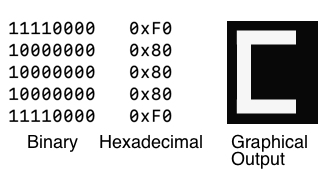
\includegraphics[scale=0.6]{images/c8_fonts_repr}
		\caption{Konwersja litery "C" z liczby binarnej do szesnastkowej i postaci graficznej}
	\end{center}
\end{figure}

Kolejną metodą klasy \textit{Memory} jest ta, odpowiedzialna za wczytanie pliku binarnego z programem. Działa ona podobnie do poprzednio przedstawionej funkcji, odpowiedzialnej za wczytywanie czcionek, z tą różnicą, że wykorzystana została wbudowana w język Python funkcja \textit{open()} z argumentem  \textit{'rb'} (\textit{read binary}), odpowiedzialnym za wczytywanie pliku w postaci binarnej. Tym razem dane są wczytywane do pamięci \textit{RAM} od adresu z indeksem 512, czyli przestrzeni specjalnie przeznaczonej na zewnętrzny program \cite{Cowgod}.

\subsection{Deasembler}
Deasembler to dodatkowy moduł zaimplementowany w celu lepszego zapoznania się z instrukcjami procesora. Podobnie jak kod odpowiedzialny za emulowanie procesora. Wczytuje on instancje klasy odpowiedzialnej za zarządzanie pamięcią, a następnie za pomocą metody \textit{get\_opcode}, przekazuje wartość do zmiennej \textit{opcode}. Następnie wydobywane są argumenty instrukcji, czyli bajty, który nie służą do rozpoznania wykonywanej operacji. Wskazują one jedynie odpowiednie numery rejestrów lub bajty które zostaną do nich dodane, a następnie przekazuje je do atrybutu \textit{args}. Kolejnym krokiem jest zamaskowanie argumentów w zmiennej trzymającej kod instrukcji, tak, aby posiadała ona informacje odpowiadające jedynie za identyfikacje kodu procesora. Otrzymane dane służą jako klucz w słowniku, jego wartością jest natomiast funkcja zwracająca podstać mnemoniczną danego \textit{słowa}. Na końcu wszystkie otrzymane informacje są odpowiednio formatowane jako zmienna typu \textit{string}. Cała procedura powtarzana jest w pętli od pierwszego adresu w pamięci do ostatniego, a licznik programu za każdą iteracją jest inkrementowany o 2.
\begin{figure}[!htb]
	\begin{center}
		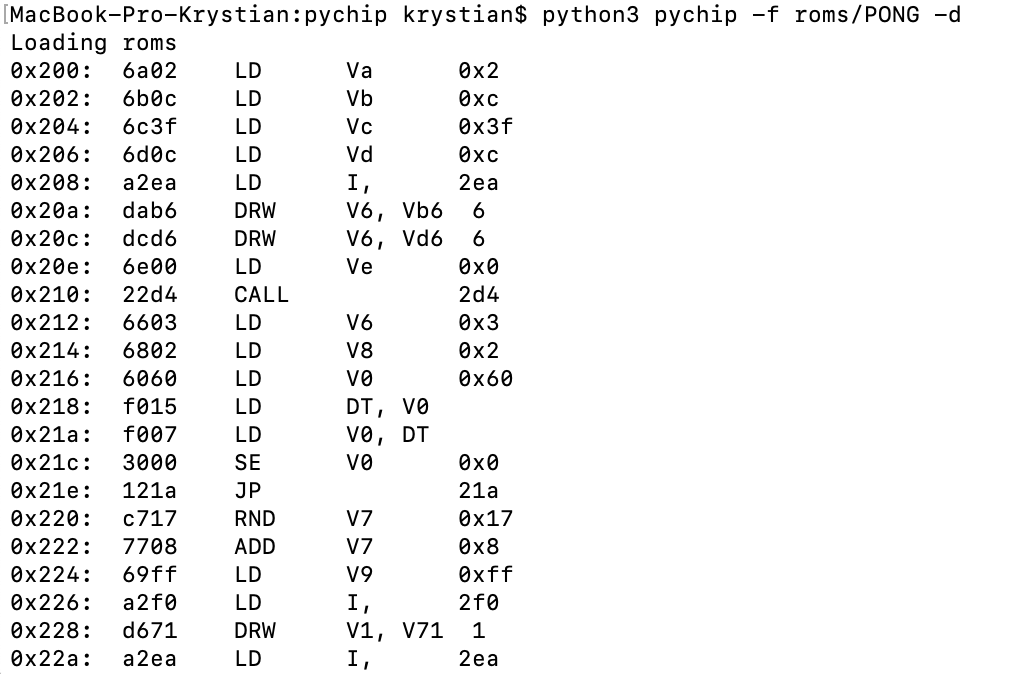
\includegraphics[scale=0.6]{images/outputDasm.png}
		\caption{Efekt działania modułu deasemblera}
	\end{center}
\end{figure}

\subsection{Moduł procesora}
Klasa \textit{Processor} przyjmuje instancje pamięci jako argument, następnie przy inicjalizacji tworzony jest słownik trzymający stan rejestrów \textit{V}, \textit{S} i \textit{I}, a także \textit{delay} i \textit{sound}. Następnie tworzone są zmienne, wskazujące na komórkę w pamięci \textit{RAM}, czyli \textit{program counter} i wskaźnik na stos \textit{stack pointer}. Kolejnymi polami są: lista odzwierciedlająca bufor ekranu i zmienna typu \textit{true/false} trzymająca informacje, czy zawartość ekranu była edytowana. Jest ona używana do sprawdzenia, czy moduł odpowiedzialny za wyświetlanie obrazu potrzebuje wygenerować na nowo grafikę. Ostatnimi atrybutami są tworzone przy inicjalizacji: \textit{pressed\_key} posiadający ostatniego klikniętego klawisza i słownik \textit{instructions}.\\

Działanie klasy procesora oparte jest o wczytywanie obecnie wskazanej przez \textit{program counter} i następnej komórki do specjalnej zmiennej nazwanej \textit{operand}. Spowodowane jest to tym, że kody procesora mają postać szesnastobitową, a pamięć jest ośmiobitowa. Z tego względu wartość \textit{operand} musi zostać przesunięta o 8 bitów w prawo, przez co do tej zmiennej dołączane jest osiem zer, następnie wykorzystuje operacje alternatywy, dzięki temu wartość z obu komórek włączana jest do zmiennej \textit{operand}. \\

Wszystkie instrukcje procesora są zaimplementowane jako funkcje. W Pythonie sama funkcja bez jej wywołania jest traktowana jako obiekt, dlatego można go wykorzystać jako wartość w słowniku, którego kluczami będą liczby od 0x0 do 0xF, odpowiadają one zakresowi starszych półbajtów pierwszych bitów instrukcji przedstawionych w \textit{Cowgod's CHIP-8 Technical Reference} \cite{Cowgod}.

\begin{lstlisting}[caption={Budowa słownika \textit{instructions}},captionpos=b]
self.instructions = {
    0x1: self.jp_addr,
    0x2: self.call_addr,
    0x3: self.se_vx_byte,
    0x4: self.sn_vx_byte,
    0x5: self.se_vx_vy,
    0x6: self.ld_vx_byte,
    0x7: self.add_vx_byte,
    0x9: self.sne_vx_vy,
    0xa: self.ld_i_addr,
    0xc: self.rnd_vx_byte,
    0xd: self.drw_vx_vy_n,
    0x0: self.sys_ops,
    0x8: self.logical_ops,
    0xf: self.rest_ops,
    0xE: self.press_ops
}
\end{lstlisting}

Po dostarczeniu wartości pamięci do zmiennej \textit{operand} wybierany jest z niej starszy półbajt pierwszego bajta, który staje się kluczem do wcześniej wspomnianego słownika \textit{instructions}. Na jego podstawie wybierana zostaje instrukcja, która będzie wykonywana. W razie gdyby taki klucz nie istniał, wykonywana jest pusta funkcja lambda, która wyświetli informacje o błędzie. Zanim to jednak się stanie, wartość licznika programu podnoszona\footnote{Wartość licznika programu inkrementowana jest za każdym razem o 2, tak aby pominąć wykorzystane już komórki, które pełnią role młodszych bajtów w zmiennej \textit{operand}} jest o 2. 

\begin{lstlisting}[caption={Framgent kodu, służący do wywoływania instrukcji procesora.},captionpos=b]
def get_operand(self):
    return self.memory[self.pc] << 8 | self.memory[self.pc + 1]

def extract_opcode(self):
    return (self.operand & 0xf000) >> 12

def execute_instruction(self):
    self.operand = self.get_operand()
    opcode = self.extract_opcode()
    self.pc += 2
    self.instructions.get(opcode, lambda x: ...)()
\end{lstlisting}

Po wykonaniu kodu operacyjnego zostaje zmieniana jeszcze wartość zegarów emulowanego urządzenia.
\subsubsection{Instrukcje}
Istnieją przypadki, gdzie pod wspomnianym wcześniej identyfikatorem można wyróżnić kilka kodów procesora, wówczas są one weryfikowane na podstawie pozostałych bitów wewnątrz jednej funkcji za pomocą instrukcji warunkowej \textit{if}. Takimi przypadkami są klucze w słowniku o wartościach: \textit{0x0}, \textit{0x8}, \textit{0xE}, \textit{0xF}.

Implementacja poszczególnych z ich wygląda następująco:

\begin{itemize}
  \item Wywołaj adres z stosu (\textit{call\_addr}):
\end{itemize}
Do rejestru \textit{S}, dodawana jest wartość \textit{licznika programu}, a \textit{wskaźnik stosu} jest inkrementowany o jeden. Następnie za pomocą operacji binarnej \textit{AND}, z wartości \textit{operand} wybieranych jest 12 ostatnich bitów. Zostają one przypisane do \textit{licznika programu}.
\begin{lstlisting}[caption={Framgent kodu, odpowiedzialny za instrukcje \textit{call\_addr}},captionpos=b]
self.registers['s'].append(self.pc)
self.sp += 1
self.pc = self.operand & 0x0fff
\end{lstlisting}

\begin{itemize}
  \item Pomiń następną instrukcje jeżeli \textit{Vx==Vy} (\textit{sne\_vx\_vy}):
\end{itemize}
Dzięki operacji binarnej \textit{AND} z pierwszego bajta \textit{słowa} wyciągane są młodsze bity. W celu usunięcia drugiego bajta wykonywane jest przesunięcie bitowe o 8. Uzyskana zmienna posłuży do identyfikacji rejestru \textit{Vx}. Następnie w podobny sposób ze \textit{słowa} wyciągana jest wartość do identyfikacji rejestru \textit{Vy}. Jeżeli wartości z rejestrów \textit{Vx} i V{y} są sobie równe, to \textit{licznik programu} inkrementowany jest o 2.
\begin{lstlisting}[caption={Implementacja instrukcji \textit{sne\_vx\_vy}},captionpos=b]
x = (self.operand & 0x0f00) >> 8
y = (self.operand & 0x00f0) >> 4
if self.registers['v'][x] == self.registers['v'][y]:
    self.pc += 2
\end{lstlisting}

\begin{itemize}
  \item Dodaj \textit{Vx} do \textit{Vy} (\textit{add\_vx\_vy}):
\end{itemize}
Wartość z rejestru \textit{Vy} jest dodawana do rejestru \textit{Vx}. Jeżeli po dodaniu \textit{Vx} przekracza 256 bitów, ustawiana jest flaga w rejestrze \textit{Vf}. Sprawdzona zmienna za pomocą instrucji \textit{AND} zostaje zredukowana do wartości mniejszej niż 256. W przeciwnym przypadku, flaga \textit{Vf} zostaje wyzerowana.
\begin{lstlisting}[caption={Implementacja instrukcji \textit{add\_vx\_vy}},captionpos=b]
self.registers['v'][x] += self.registers['v'][y]
if self.registers['v'][x] > 0xFF:
    self.registers['v'][0xF] = 1
    self.registers['v'][x] &= 0xFF
else:
	self.registers['v'][0xF] = 0
\end{lstlisting}


\newpage

\subsection{Moduł wejścia/wyjścia}
Podstawą tego modułu jest klasa \textit{Window}, dziedzicząca z\textit{tkinter.Tk}. Odpowiada ona za podstawę interfejsu użytkownika wyświetlającego emulacje, jego konfiguracje, a także pasek menu przy górnej belce. Przy jej inicjalizacji zostaje ustalony rozmiar okna, a także zablokowana możliwość ręcznego zmieniania jego wielkości. Następnie zostaje ustalona kolejność komend na pasku narzędzi. Pierwszą opcją jest \textit{file}, w której zawiera funkcja \textit{open}. Odpowiedzialną za wywołanie okna wyboru pliku. Jest to standardowy \textit{dialog} z pakiety \textit{tkinter.filedialog} \cite{TKINTER}.

\begin{figure*}[!htb]
\begin{center}
	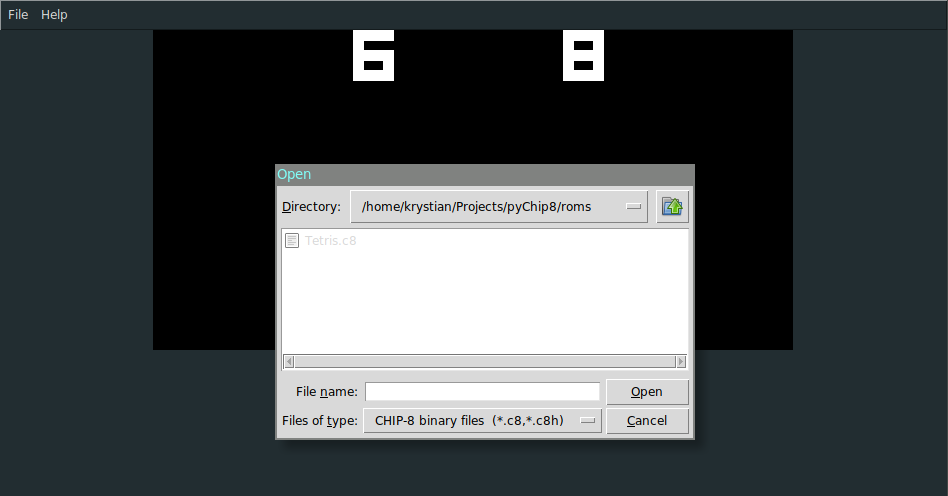
\includegraphics[scale=0.32]{images/fileDialog}
	\caption{Dialog do wybierania plików (system \textit{GNU/Linux })}
\end{center}
\end{figure*}

 W opisywanym projekcie potrzebne były różne konfiguracje dla każdej ze wspieranych platform. Dla przykładu system windows do przedstawienia ścieżek używa znaku \textit{lewego ukośnika}, gdy w platformach \textit{uniksowych} jest to zwykły ukośnik. Dodatkowo \textit{dialog} w systemie\textit{macOS}  wyświetlający pliki nie posiada możliwości wyboru formatu, więc w tym przypadku, trzeba było pozostawić opcję wyboru tylko wszystkich plików.
 
\begin{figure*}[!htb]
\begin{center}
	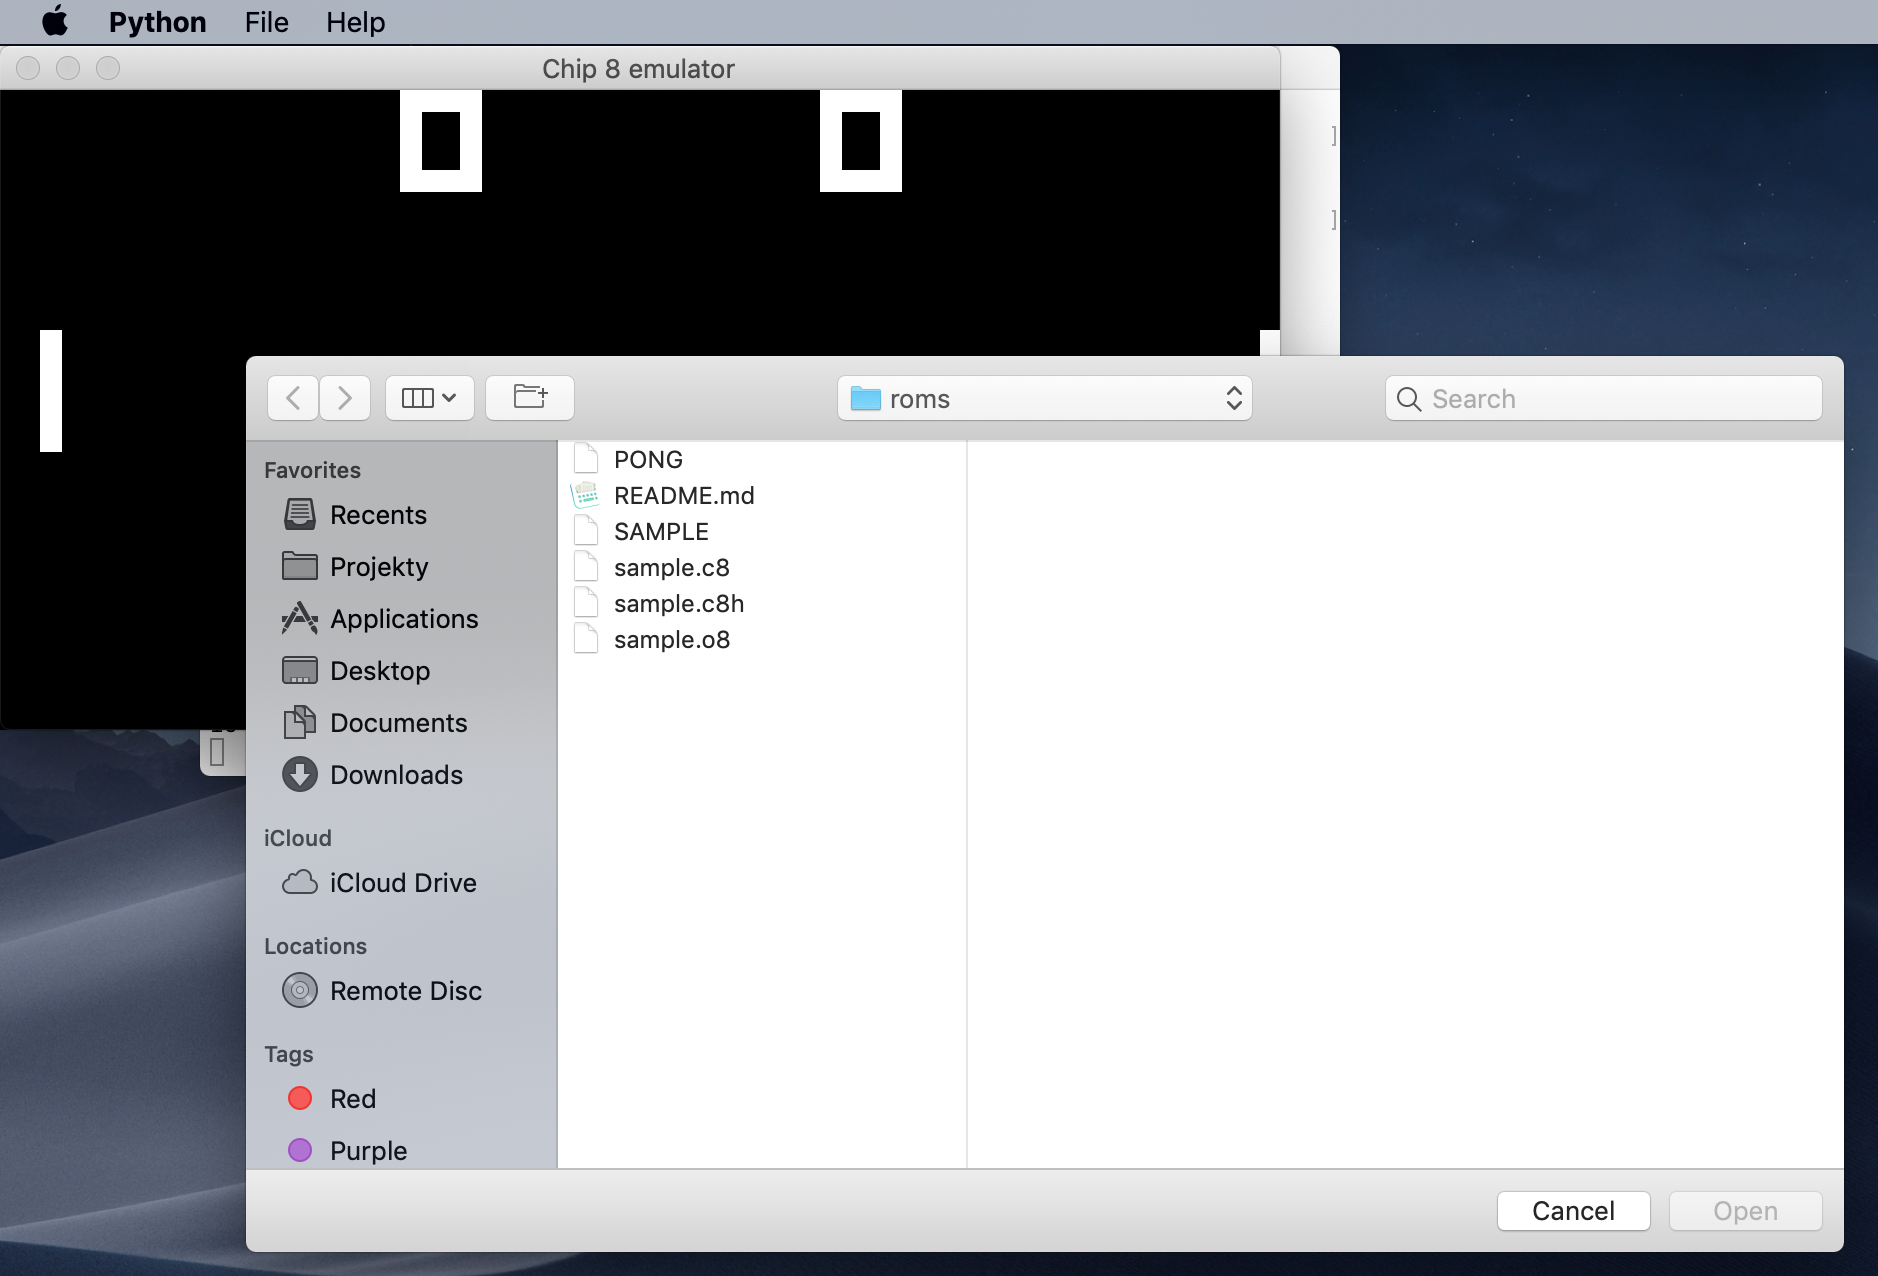
\includegraphics[scale=0.3]{images/fileDialog-macos}
	\caption{Dialog do wybierania plików (system \textit{macOS})}
\end{center}
\end{figure*}

\newpage

Kolejną opcją jest \textit{reset}, gdzie przywracane są wszystkie rejestry do wartości początkowych, a emulacja rozpoczyna się na nowo. Następną sekcją jest \textit{help}, która zawiera opcje \textit{about}, w których są zawarte informacje o wersji programu z linkiem do \textit{githuba} projektu i \textit{changelog}, gdzie opisano zmiany w wersja. We wszystkich tych przypadkach skorzystano z modułu \textit{tkinter.messagebox} \cite{TKINTER}, który wyświetla okienka informacyjne. System \textit{macOS} posiada pasek menu, który zmienia się zależnie od aplikacji przez co, nie ma pojawia się pasek narzędzi w okienku aplikacji. Ma on dodatkową sekcje, która ma taką samą nazwę jak ta aplikacji. Z tego względu dla tej platformy dodano funkcję, która zmienia wyświetlane w nim informacje na te z sekcji \textit{about}.


\begin{figure*}[!htb]
\begin{center}
	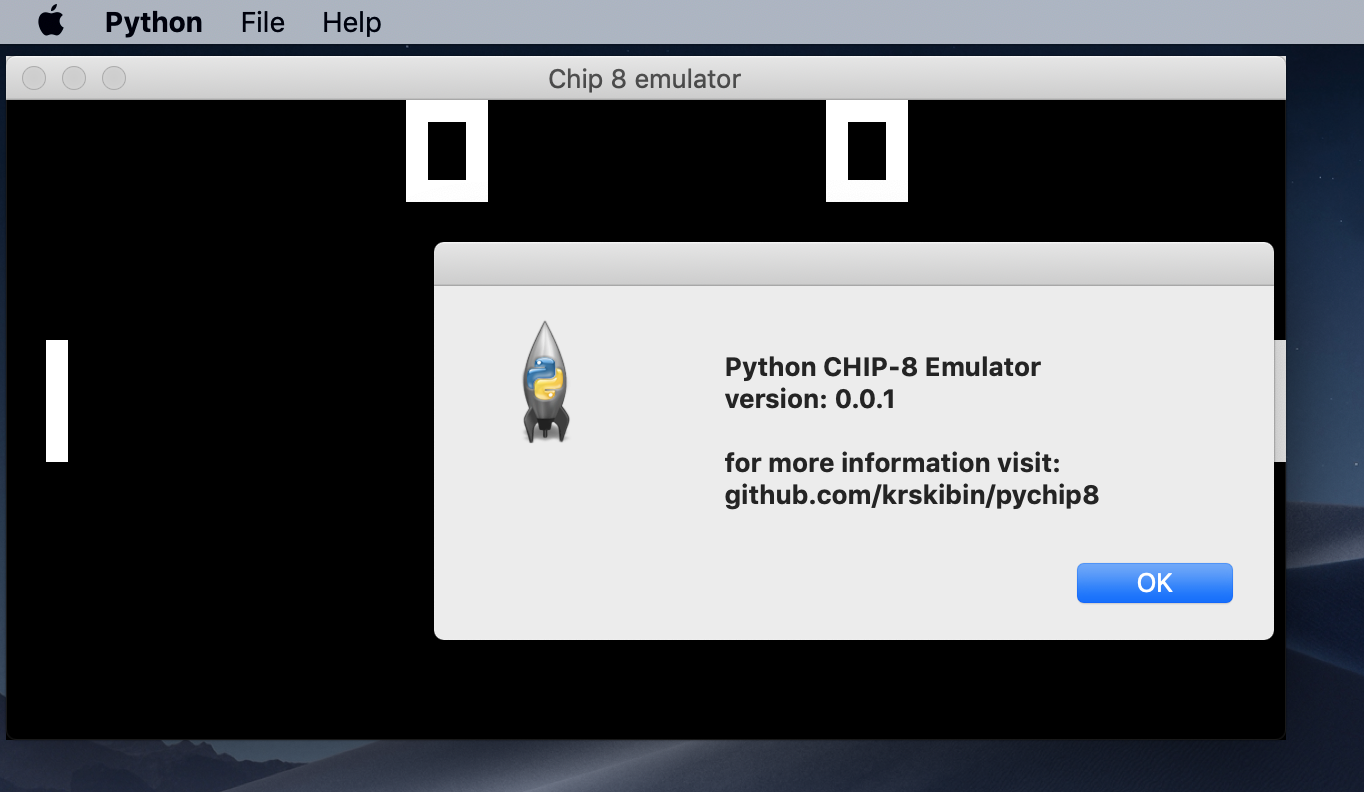
\includegraphics[scale=0.4]{images/aboutSection}
	\caption{\textit{Messagebox} z informacjami (system macOS)}
\end{center}
\end{figure*}

Następnym zaimplementowanym fragmentem kodu jest klasa \textit{Screen}. Odpowiada ona za sterownie wcześniej opisaną klasę \textit{Window}. To przy jej inicjalizacji podpinane są zdarzenia dla kliknięcia klawisza. Są to funkcje:\textit{key\_down} i \textit{key\_up}. Ich zadaniem jest mapowanie klawiszy z klawiatury użytkownika na heksadecymalną, którą oryginalnie obsługiwały komputery dla których był napisany CHIP-8 \cite{COSMAC}.

\begin{lstlisting}[caption={Słownik z mapowaniem klawiszy (wartości w nawiasach, to rzeczywiste klawisze)},captionpos=b]
self.keymap = {
   '1': 1, '2': 2, '3': 3, '4': 12, 'q': 4, 'w': 5,
   'e': 6, 'r': 13, 'a': 7, 's': 8, 'd': 9, 'f': 14,
   'z': 10, 'x': 0, 'c': 11, 'v': 15,
}
\end{lstlisting}
Do tej klasy podpięto również obiekt \textit{tkinter.Canvas} \cite{TKINTER}, który dostarcza interfejs pozwalający na rysowanie kształtów. Wykorzystuje ją metoda  \textit{draw\_pixel}, której zadaniem jest iteracja po \textit{buferze} z modułu procesora i gdy napotka wartość \textit{1}, to w tym miejscu, na odpowiednie przeskalowanym kanwasie rysuje kwadrat. Dla oszczędzenia pamięci, przed wywałniem tej metody, wszystkie obiekty z kanwasu są usuwane. Ostatnią metodą w tym module jest ta odpowiedzialna za czyszczenie ekranu emulatora. Jest ona interfejsem do metody zaimplementowanej w \textit{tkinter} i przyjmuje ona specjalną stałą \textit{tkinter.ALL} zawierającą referencje do każdego obiektu kanwasu.


\subsection{Główny moduł programu}

Jest to moduł odpowiedzialny za ciągłe działanie emulatora. Tworzone są w nim instancje zaimplementowanych klas, a także przekazane wymagane argumenty. Następnie ustalana jest rozdzielczość ekranu, obecność dźwięku i szybkość działania procesora. Kolejnym krokiem jest rozpoczęcie \textit{głównej pętli aplikacji}, która z każdą iteracją wykonuje kolejną instrukcje procesora, a także definiuje jego prędkość taktowania.
\begin{figure*}[!htb]
\begin{center}
	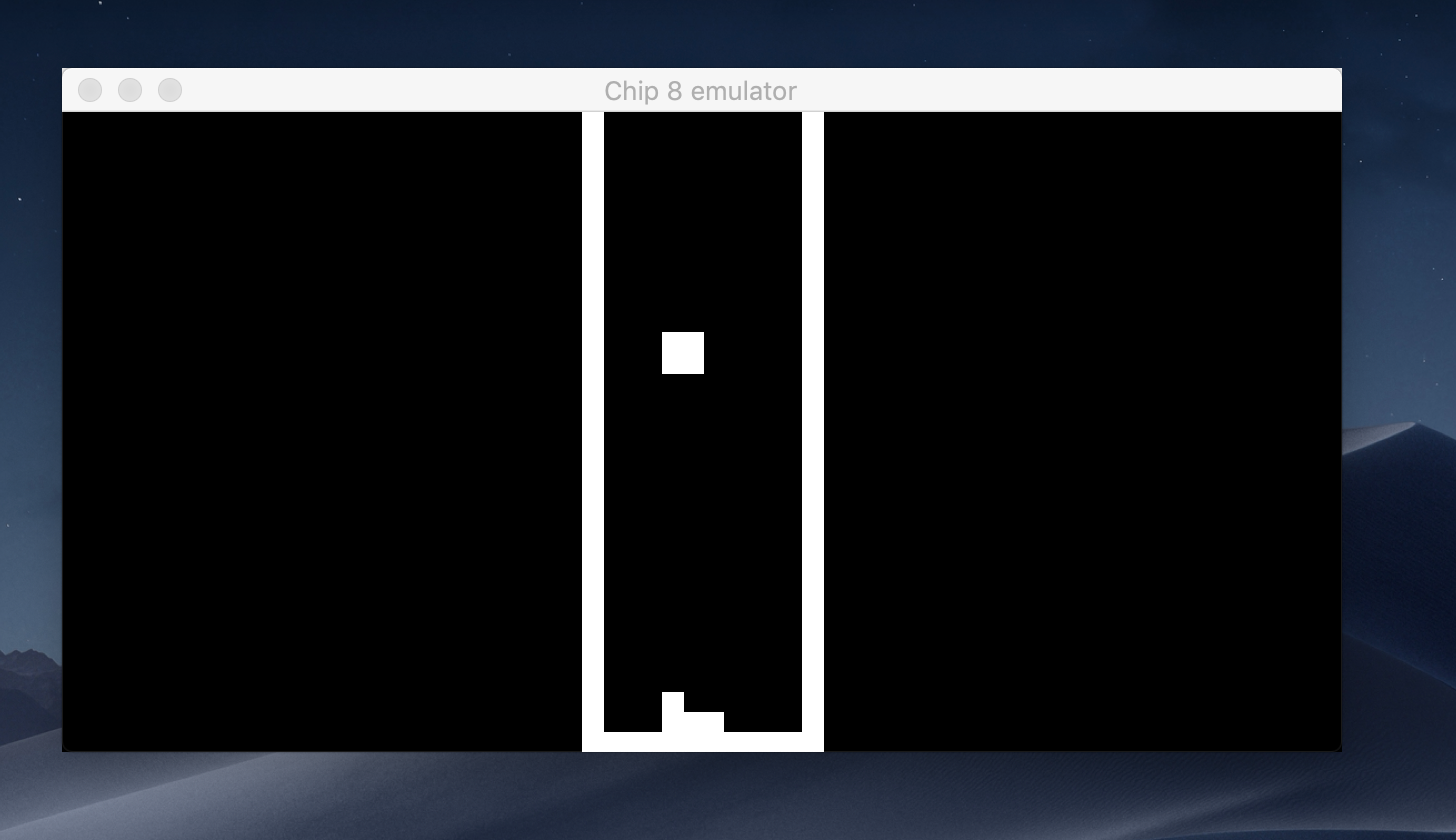
\includegraphics[scale=0.4]{images/workingApp}
	\caption{Działający emulator, gra \textit{TETRIS} (autor Fran Dachille, rok 1991)}
\end{center}
\end{figure*}

W module znajduje się również implementacja interfejsu linii poleceń. Jest to obiekt z pakietu \textit{argparse}, który za pomocą metody \textit{add\_argument} \cite{Argparse}, definiuje opcje, przyjmowane przez program przy wywołaniu, a także ich opis, typ i nazwy zmiennych do których zostaną przepisane  one w kodzie aplikacji.

\begin{lstlisting}[caption={Wynik uruchomienia programu z opcją \textit{-h}},captionpos=b]
$../pychip: python pychip -h
usage: [-h] [-f ROMS] [-d] [-r RES] [-t DLY]

Chip8 emulator

optional arguments:
  -h, --help            show this help message and exit
  -f ROMS, --file ROMS  use to provide roms file
  -d, --disassembler    run disassembler for given roms file
  -r RES, --res RES     set CHIP-8 screen resolution
  -t DLY, --time DLY    set emulation delay time

\end{lstlisting}







\section{Testy}
Projekt był tworzony zgodnie z techniką \textit{programowania sterowanego testami (ang. \textit{test driven development})} \cite{WOZNIAK}. W związku z tym, przed napisaniem jakiejkolwiek fragmentu kodu najpierw opracowywany był dla niego test. To podejście pomaga utrzymać większą jakość kodu, a także pozwala na szybsze wykrycie, czy dana funkcja zwraca pożądaną wartość lub odpowiednio modyfikuje zmienne. W takim projekcie jak emulator, gdzie najmniejsze odchylenie w generowanych przez program wartościach może sprawić, że emulowany program będzie działał niezgodnie z oczekiwaniami, testy przydają się jako narzędzie wspierające debugowanie kodu.\\

Twórcy \textit{Pythona} w bibliotece standardowej zapewnili pakiet \textit{unittest} odpowiedzialny za testy, jednak w projekcie został użyty \textit{pytest} ze względu na większą ilość narzędzi przydatnych przy pisaniu testów dla dużej ilości danych wejściowych.\\

Ilość interakcji w programie jest mała, a ich każdorazowe wystąpienie bezpośrednio wpływa na stan programu, dlatego uznano, że testy integracyjne i akceptacyjne \cite{WOZNIAK} nie są potrzebne, a do przetestowania aplikacji wystarczą testy jednostkowe.\\

Strukturę testu jednostkowego definiuje zasada \textit{Arrange-Act-Assert} \cite{WOZNIAK}. Na samym początku wszystkie dane  są przygotowywane (arrange) i odizolowywane. Ważne, aby zewnętrzne zależności, takie jak inne klasy, czy obsługa strumieni wejścia i wyjścia zastąpione były atrapami (ang. \textit{mock}). Jest to główna różnica między podejściem jednostkowym, a modułowym, gdzie tego typu zależności są dopuszczalne. Następnym krokiem jest wykonanie działania na testowanym fragmencie kodu (\textit{act}) i sprawdzenie, czy jego wywołanie zwróciło porządny rezultat (\textit{assert}). Przeważnie biblioteki testowe dostarczają odpowiednią funkcjonalność do porównywania danych oczekiwanych z tymi, które są przetwarzane przez sprawdzany fragment programu. Inaczej jest w przypadku modułu \textit{pytest}, który dokonuje tego wykorzystując wbudowaną w język Python funkcję \textit{assert} \cite{PYTEST}. Jej działanie jest podobne do standardowej instrukcji \textit{if} z tą różnicą, że niespełnienie warunku od razu traktowane jest jako błąd \cite{PYTEST}. 
\begin{lstlisting}[caption={Przykład prostego testu przy użyciu biblioteki \textit{pytest}},captionpos=b]
class TestProcessor:
	def test_reset(self):
		"""
		Processor.reset() powinien ustawic pointer counter
		do domyslnej wartosci (0x200)
		"""
		# arrange
		proc = Processor()
		proc.pc = 0x230
		
		# act
		proc.reset()
		
		# assert
		assert self.pc == 0x200
\end{lstlisting}
Kolejnym ważnym komponentem \textit{pytestu} jest parametryzacja testów. Zapewnia ona dostarczenie różnych danych wejściowych i oczekiwanych wyników bez potrzeby tworzenia testów dla innych przypadków \cite{PYTEST}.
\begin{lstlisting}[caption={Przykład testu sparametryzowanego.},captionpos=b]
class TestDisasssembler:
    mask_params = ([0xFDEE, 0xF0EE], [0xE337, 0xE037],
                   [0x0ABC, 0x00BC], [0x8DCA, 0x800A], 
                   [0xAACE, 0xA000])

    @pytest.mark.parametrize(("opcode", "expected"), mask_params)
    def test_opcode_mask(self, opcode, expected):
        dasm = Disassembler()
        assert dasm.mask_opcode(opcode) == expected
\end{lstlisting}
W obu listingach wewnątrz każdego testu jest tworzony nowy obiekt klasy, do której należy sprawdzana funkcja. Procedurę tę można zautomatyzować, tworząc tak zwane \textit{fixture} \cite{PYTEST}. Są to najczęściej funkcje, których zadaniem jest automatyczne wykonanie się zanim zależne od nich testy zostaną rozpoczęte.
\begin{lstlisting}[caption={Przykład poprzedniego testu z użyciem \textit{fixture}.},captionpos=b]
@pytest.fixture(scope="function")
def dasm(request):
    return Disassembler()

@pytest.mark.usefixtures('dasm')
class TestDisassembler:
    # ...
    
    @pytest.mark.parametrize(("opcode", "expected"), mask_params)
    def test_opcode_mask(self, opcode, expected, dasm):
        assert dasm.mask_opcode(opcode) == expected
\end{lstlisting}
Jak już wcześniej zostało wspomniane, testy jednostkowe nie mogą korzystać z zewnętrznych zależności potrzebnego do utworzenia sprawdzanej klasy lub funkcji. Zamiast nich tworzymy obiekty atrapy. Imitują one jedynie rzeczywistą instancje klasy, jej atrybutu, jak również ich wywołania. W przypadku tego projektu wykorzystano moduł z biblioteki standardowej \textit{unittest.mock}. Dostarcza ona klasę \textit{MagicMock}, jej zadaniem jest tworzenie imitacji obiektów, wtedy, kiedy test wymaga dostępu do ich metod lub atrybutu \cite{MOCK}. Następnie za pomocą \textit{patch} można imitować pola lub funkcje wybranej klasy \textit{MOCK} i nadawać im zwracane wartości.
\begin{lstlisting}[caption={Przykład przykład testowania za pomocą atrap}, captionpos=b]
pytest.fixture(scope="function")
def proc(request):
    memory = mock.MagicMock()
    processor = Processor(screen)
    return processor
    
class TestProcessor:
    extract_params = ([0x0523, 0x0], [0x1fcd, 0x1], [0x2cde, 0x2])
    @pytest.mark.parametrize(("operand", "expected"), extract_params)
    def test_extract_opcode(self, operand, expected, proc):
    mod = f"{self.module_name}.operand"
    with mock.patch(mod, new_callable=mock.PropertyMock) as mock_op:
       mock_op.return_value = operand
       assert proc.extract_opcode() == expected
\end{lstlisting}

Technika programowania sterowanego testami zapewniła, że od samego początku wdrażania projektu, jego kod był lepszej jakości i łatwiejszy do utrzymywania. Filozofia ta skupia dużą uwagę, na tym, aby każdy fragment programu nadawał się do przetestowania, co pozwalało na szybkie zweryfikowanie, w której części emulatora zwracał niewłaściwe rezultaty. Atrapy przyczyniły się do jeszcze większej izolacji poszczególnych modułów, co gwarantowało, że niepowodzenie danego testu zależało wyłącznie od sprawdzanej funkcji. Dzięki, parametryzacji, możliwe było przebadanie wielu danych wejściowych i porównanie, czy wszystkie zwracają porządny rezultat. To z kolei, pomagało znajdować wartości, których problematyczności nie uwzględniono w pierwszych iteracjach kodu programu.

\section{Podsumowanie}
W ramach niniejszej pracy powstał program pozwalający na wczytywanie gier z zewnętrznych plików, a następnie ich emulację, wyświetlanie w środowisku graficznym i interakcję. Na potrzebę użytkownika dowolna jest manipulacja parametrami aplikacji, tak, aby dostosować prędkość działania procesora lub skalę grafiki. Możliwe jest wybieranie innych plików do emulacji za pomocą zawartego w interfejsie graficznym paska menu, lub ich resetowanie.

Emulator uruchamia wszystkie programy opracowanych na maszynę wirtualną~{CHIP-8}.

Projekt w całości spełnia przyjęte wymagania i został opracowany zgodnie z przeprowadzonymi założeniami projektowymi i specyfikacją maszyny wirtualnej \cite{Cowgod}.


\subsection{Możliwe udoskonalenia}
Dalszy rozwój emulatora powinien opierać się na zaimplementowaniu instrukcji dla \textit{Super CHIP-48} \cite{Cowgod}, czyli ulepszonej wersji CHIP-8. Tu potrzebne byłoby również opracowanie ulepszonego mechanizmu wyświetlania grafiki i dodanie przewijania ekranu \cite{Cowgod}. Dobrym pomysłem wydaje się zaimplementowanie \textit{debuggera}, który podświetlałby aktualnie wykonywaną instrukcję w oknie i dawał możliwość ich wykonywania krok po kroku lub cofania, przy okazji wyświetlając w innym miejscu aktualny stan rejestrów. W kwestii zupełnie nowych funkcji można byłoby dodać moduł odpowiedzialny za kompilowanie specjalnie utworzonej odmiany \textit{języka assemblera} do plików, które wczytywałby emulator. Umożliwiałoby to tworzenie własnoręcznie napisanych gier pod tę platformę.

\newpage

\bibliographystyle{plain}
\bibliography{bibliografia}

\end{document}
